\section{Measurement}

In the present section, we will perform some measurements with the \gls{psd}.
In particular, we want to determine the spatial resolution and discuss the noise characteristics.

\subsection{Electrical setup}

\Cref{tab:equipment} lists the equipment required for the electrical setup.
The electric devices are connected as follows.
The \gls{psd} is connected with the power supply through the LEMO4 cable.
The DIFFX, DIFFY, and SUM output voltages of the \gls{psd} are conencted to the oscilloscope's first three input channels.
It is essential to use shielded cables to avoid receiving \SI{50}{\hertz} noise from surroudning switching power supplies.

\begin{table}[htb]
  \centering
  \begin{tabular}{ccl}
    \toprule
      Device & Amount \\
    \midrule
      \gls{psd} & 1\\
      Oscilloscope & 1\\
      \SI{\pm15}{\volt} voltage supply & 1\\
      Shielded LEMO4 cable & 1\\
      Shielded \acrshort{sma} cable & 3\\
      \acrshort{sma} to \acrshort{bnc} adapters & 3\\
    \bottomrule
  \end{tabular}
  \captionsetup{width=.8\textwidth}
  \caption{Electrical equipment required to operate the \gls{psd}}\label{tab:equipment}
\end{table}

You can configure the oscilloscope to show the first two input channels in X-Y mode.
In X-Y mode, the signal on the coordinate grid corresponds to the position of the incident light spot.
Suppose your light source shows strong intensity fluctuations.
In that case, you can use the oscilloscope's arithmetic operation to divide the DIFFX and DIFFY signals by the SUM signal.

\subsection{Optical setup}

\Cref{fig:optical_setup} shows an optical setup for spatial resolution measurements.
The arrangement comprises a laser source, two mirrors, a lens with focal length $f=\SI{50}{\milli\meter}$ positioned in \SI{11}{\centi\meter} distance from the \gls{psd}.
Using two mirrors instead of one allows more freedom in positioning the other optics.
The lens focuses the laser beam onto the sensitive area of the \gls{psd}.
\begin{figure}[htb]
	\centering
	\includestandalone[mode=buildnew]{figure/optic/setup}
	\caption{Optical setup for testing}\label{fig:optical_setup}
\end{figure}
We measured an optical power of $P=\SI{1}{\milli\watt}$ for the red laser at $\lambda=\SI{700}{\nano\meter}$ with the optical power meter.

\subsection{Grid scan}

\begin{figure}[H]
	\centering
	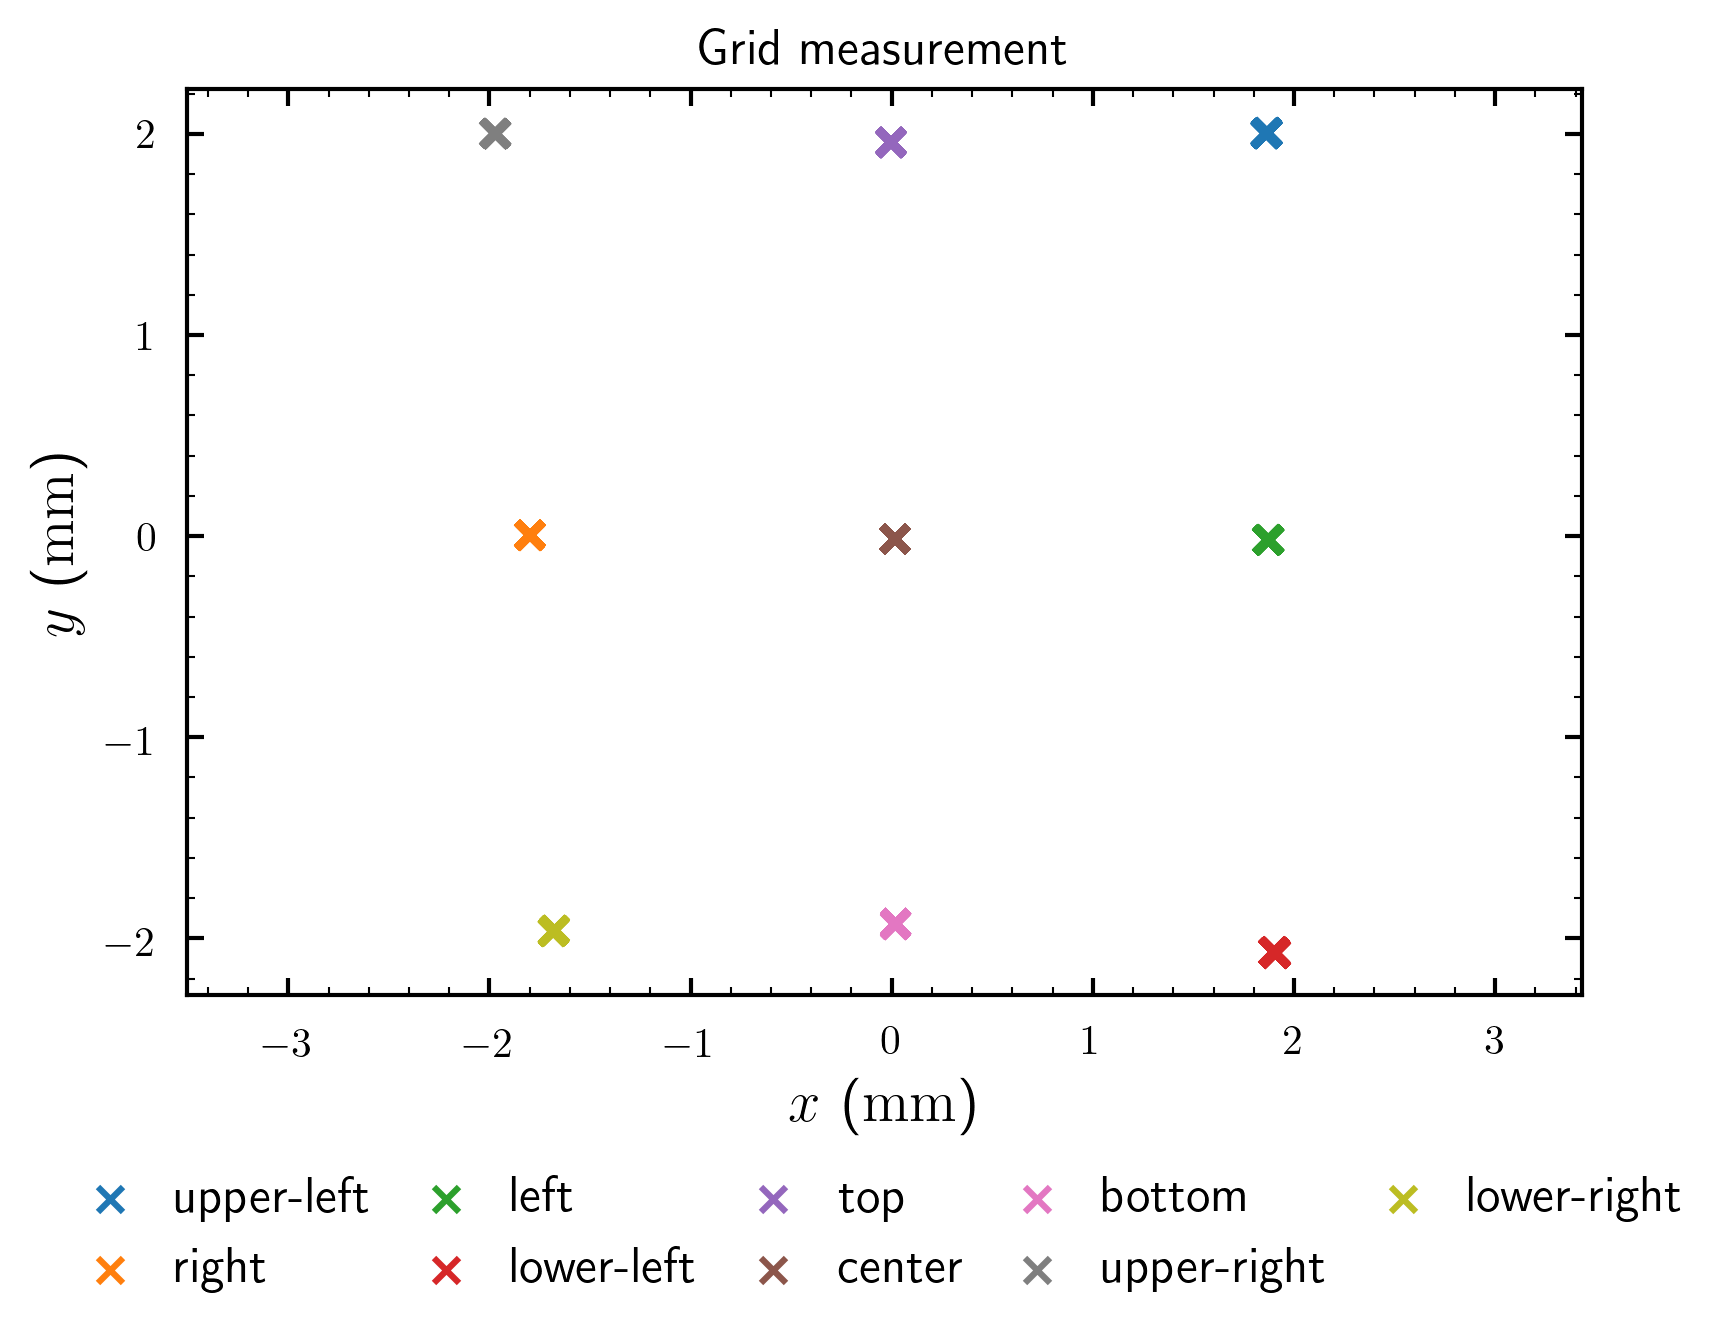
\includegraphics{figure/plot/grid-measurement}
	\caption{Spatial scan over $3\times 3$ grid by adjusting the mirrors.}\label{fig:grid_scan}
\end{figure}
\Cref{fig:grid_scan} shows the positions of a 3 x 3 grid scan.
We adjusted mirror M2 in the optical setup shown in \cref{fig:optical_setup} and captured a trace with the oscilloscope.
In the post-processing, we converted the captured voltages to positions.
The datasheet of the S5990 position-sensitive photodiode gives a conversion formula for the photocurrents
\begin{align}
	\frac{(I_2+I_3)-(I_1+I_4)}{I_1+I_2+I_3+I_4}=\frac{2x}{L},
	&&
	\frac{(I_2+I_4)-(I_1+I_3)}{I_1+I_2+I_3+I_4}=\frac{2y}{L}
	\label{eq:position_conversion_photocurrent},
\end{align}
wherein $L$ is the length of the photodiode's quadratic sensitive area.
In our case, we have the smaller S5991-01 photodiode where $L = \SI{4}{\milli\meter}$.
In terms of the output voltage signals of the \gls{psd}, the positions are then given by
\begin{align}
	x=\frac{L}{2}\frac{\text{DIFFX}}{\text{SUM}}\ \si{\milli\meter}, &&
	y=\frac{L}{2}\frac{\text{DIFFY}}{\text{SUM}}\ \si{\milli\meter}.
	\label{eq:position_conversion_voltages}
\end{align}

\subsection{Resolution}

\begin{figure}[htb]
	\centering
	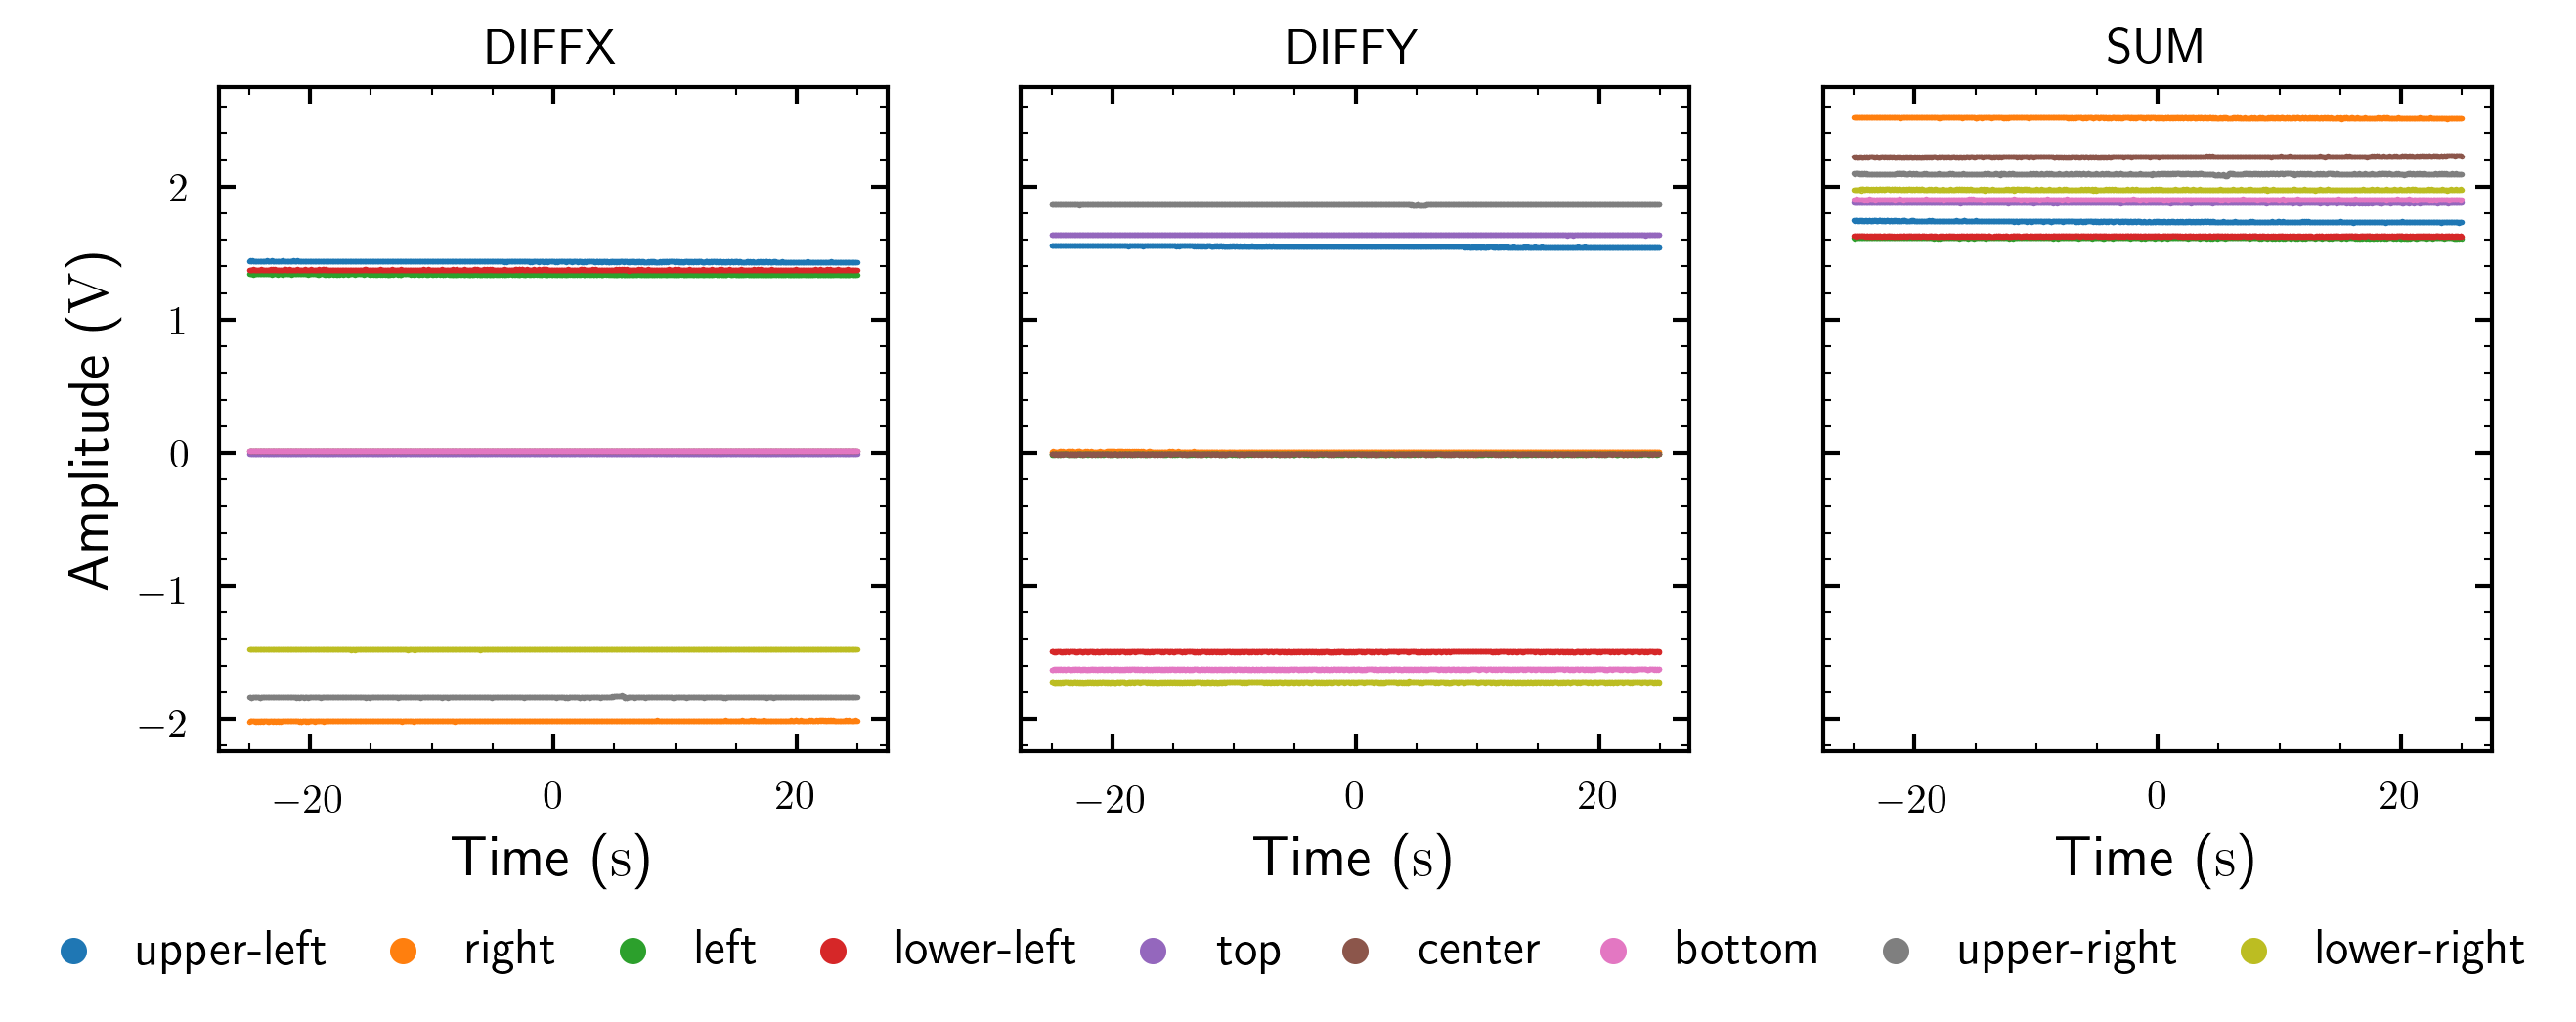
\includegraphics[scale=0.7]{figure/plot/voltages}
	\caption{Timeseries of the voltage signals captured during the grid scan.}\label{fig:grid_scan_voltages}
\end{figure}
\Cref{fig:grid_scan_voltages} shows the voltage signals for the grid scan measurement.
The change of the SUM signal for the different measurements indicates a change in the total intensity of the detected light.
We note that the difference signals span a voltage range from \SI{-2}{\volt} to \SI{+2}{\volt}.

\begin{figure}[htb]
	\centering
	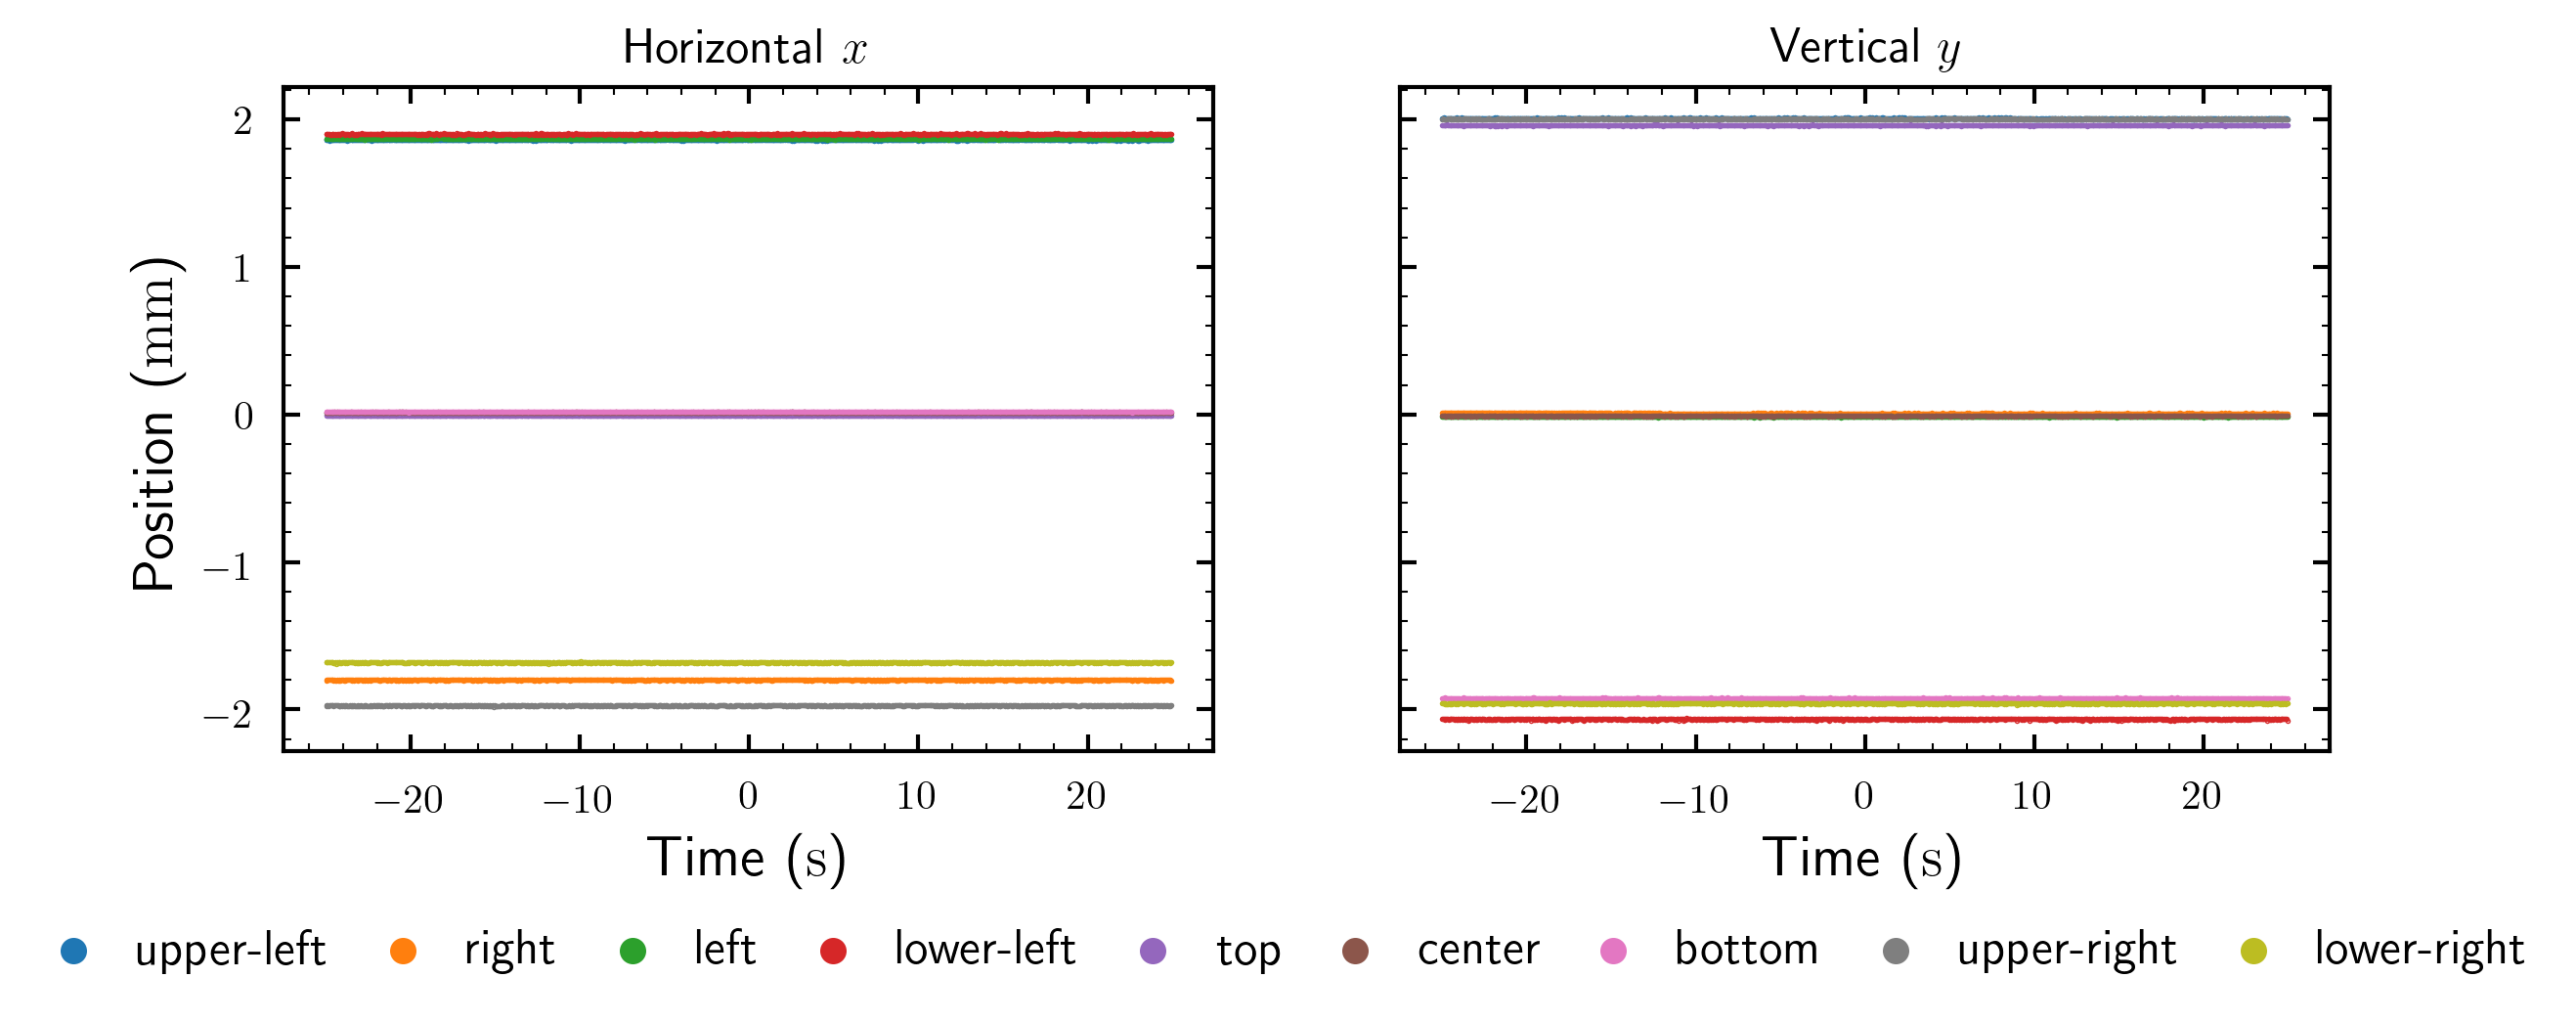
\includegraphics[scale=0.7]{figure/plot/positions}
	\caption{Voltage signals of the grid scan converted to positions.}\label{fig:grid_scan_positions}
\end{figure}
\Cref{fig:grid_scan_positions} shows the positions obtained from the voltages signals after using \cref{eq:position_conversion_photocurrent}.
Horizontal and vertical axis span an area of close to \SI{4}{\milli\meter} in agreement with the specified length of the sensitive area of the S5991-01.
We explain small deviations by the fact that we cannot precisely control the mirror adjustments.

\Cref{tab:grid_scan_position_statistics} summarizes the statistics, mean and standard deviation, of the position traces illustrated in \cref{fig:grid_scan_positions}.
For different grid positions, we find different positional uncertainty.
The highest resolution with about \SI{1}{\micro\meter} is obtained close to the center.
This is in agreement with our theoretical discussion of the position-sensitive photodiode designs where we claimed that non-linear effects become notable close to the border of the sensitive area.
\begin{table}[htb]
  \centering
  \begin{tabular}{lcccc}
    \toprule
      Measurement &
      $x$ (\si{\milli\meter}) &
      $\Delta x$ (\si{\micro\meter}) &
      $y$ (\si{\milli\meter}) &
      $\Delta y$ (\si{\micro\meter}) \\
    \midrule
      Center & \num{0.01} & \num{+1.08} & \num{-0.01} & \num{+1.03} \\      
      Top & \num{-0.01} & \num{+1.30} & \num{+1.96} & \num{+1.67} \\      
      Left & \num{1.87} & \num{+2.19} & \num{-0.01} & \num{+1.50} \\      
      Right & \num{-1.80} & \num{+1.38} & \num{+0.01} & \num{+1.61} \\
      Bottom & \num{0.02} & \num{+1.24} & \num{-1.92} & \num{+2.11} \\
      Upper left & \num{+1.86} & \num{+2.03} & \num{+2.01} & \num{+2.50} \\
      Upper right & \num{-1.97} & \num{+1.75} & \num{+2.00} & \num{+1.65} \\
      Lower left & \num{+1.90} & \num{+2.26} & \num{-2.07} & \num{+2.56} \\
      Lower right & \num{-1.68} & \num{+1.78} & \num{-1.96} & \num{+1.87} \\
    \bottomrule
  \end{tabular}
  \captionsetup{width=.8\textwidth}
  \caption{Position statistics of $3\times 3$ grid scan}\label{tab:grid_scan_position_statistics}
\end{table}

\subsection{Dark noise}

For completeness, we performed a measurement of the detector where the sensitive area is blocked.
\Cref{tab:dark_statistics} summarizes the statistics of the measurement.
\begin{table}[htb]
  \centering
  \begin{tabular}{lcc}
    \toprule
      Signal &
      Mean (\si{\milli\volt}) &
      Standard deviation (\si{\micro\meter}) \\
    \midrule
      DIFFX & \num{0.1} & \num{17} \\
      DIFFY & \num{0.4} & \num{17} \\
      SUM & \num{1.2} & \num{32} \\
    \bottomrule
  \end{tabular}
  \captionsetup{width=.8\textwidth}
  \caption{Signal statistics obtained without illumination}\label{tab:dark_statistics}
\end{table}
The variance of the voltage signals without illumination are much less than with illumination.
It is difficult to distinguish the electronic from the detector noise.

\subsection{Gaussian beam waist}

Finally, we want to compare the focused beam waist to the positional uncertainty of \cref{tab:grid_scan_position_statistics}.

In Gaussian beam optics, we define the Rayleigh length
\begin{equation}
	z_R=\frac{\pi w_0^2}{\lambda}
	\label{eq:rayleigh_length}.
\end{equation}
Using a white paper, a pen, and a ruler, we estimated the spot size in front of the lens in \cref{fig:optical_setup} to be less than $w_0=\SI{3}{\milli\meter}$.
For simplicity, we assume $\lambda=\SI{700}{\nano\meter}$ as the laser wavelength, and estimate the Rayleigh length to be $z_R=\SI{40}{\meter}$.

Consider a Gaussian beam with initial beam waist $w_0$ and Rayleigh length $z_R$ propagating through a thin lens with focal length $f$.
After a distance of $s$, the beam waist of the Gaussian beam has the size
\begin{equation}
	w^\prime_0=\frac{w_0}{\sqrt{(1-s/f)^2+(z_R/f)^2}}
	\label{eq:beam_waist_thin_lens}.
\end{equation}
For the optical setup given in \cref{fig:optical_setup}, $z_R=\SI{40}{\meter}$, $w_0=\SI{3}{\milli\meter}$, $s=\SI{11}{\centi\meter}$, $f=\SI{50}{\milli\meter}$, \cref{eq:beam_waist_thin_lens} yields $w^\prime_0=\SI{4}{\micro\meter}$.
A beam waist of \SI{4}{\micro\meter} is four times the estimated position uncertainty at the center of the \gls{psd}.
We conclude that it is unlikely for the position uncertainty to be related to the spot size.
